% OSP SMA 2019 Essay 5
\section{Soal}
Diberikan segitiga $ABC$, dengan $AC > BC$, dan lingkaran luarnya yang berpusat di $O$. Misalkan $M$ adalah titik pada lingkaran luar segitiga $ABC$ sehingga $CM$ adalah garis bagi $\angle ACB$. Misalkan $\Gamma$ adalah lingkaran berdiameter $CM$. Garis bagi $\angle BOC$ dan garis bagi $\angle AOC$ memotong $\Gamma$ berturut-turut di $P$ dan $Q$. Jika $K$ adalah titik tengah $CM$, buktikan bahwa $P, Q, O, K$ terletak pada satu lingkaran.

\begin{center}
\definecolor{uququq}{rgb}{0.25098039215686274,0.25098039215686274,0.25098039215686274}
\definecolor{xdxdff}{rgb}{0.49019607843137253,0.49019607843137253,1}
\definecolor{sqsqsq}{rgb}{0.12549019607843137,0.12549019607843137,0.12549019607843137}
\definecolor{dcrutc}{rgb}{0.8627450980392157,0.0784313725490196,0.23529411764705882}
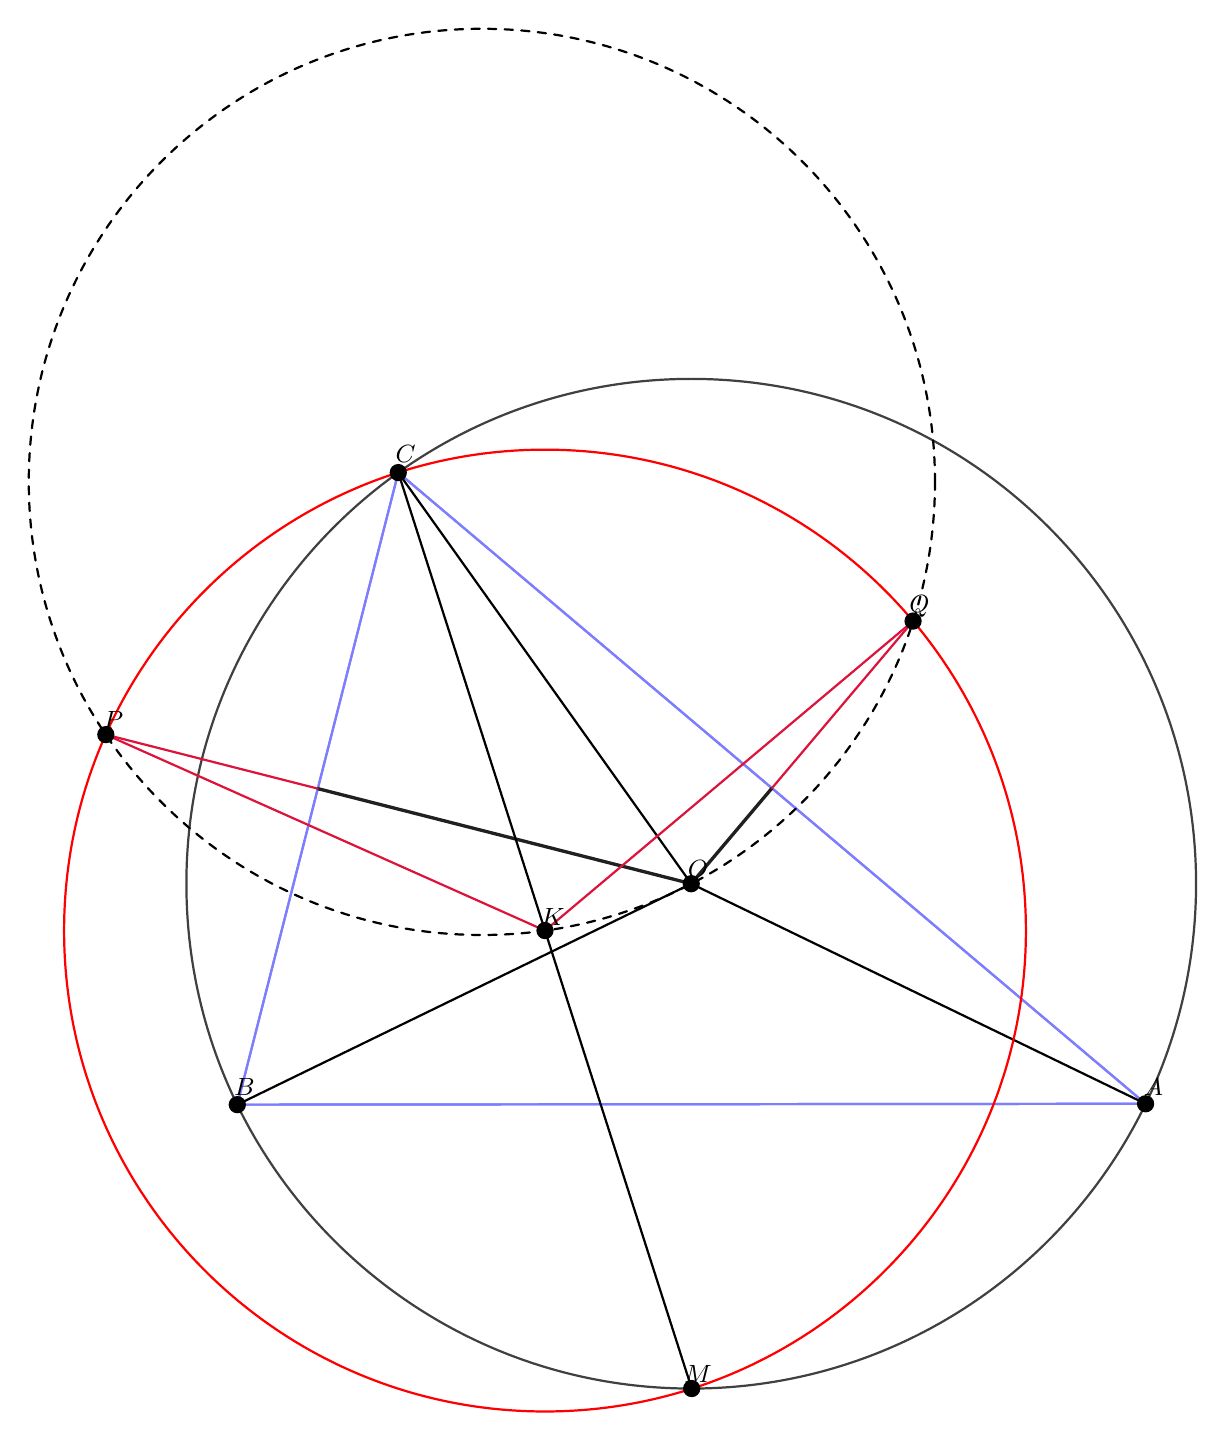
\begin{tikzpicture}[scale=2.4,line cap=round,line join=round]
  \draw[line width=0.80pt,color=xdxdff] (2.40424,-1.16441)--(-2.40199,-1.16905)--(-1.55015,2.1756)--cycle;
  \draw[line width=0.80pt,color=uququq] (0,0) circle (2.67137);
  \draw[line width=0.80pt,color=xdxdff] (2.40424,-1.16441)--(-2.40199,-1.16905);
  \draw[line width=0.80pt,color=xdxdff] (-2.40199,-1.16905)--(-1.55015,2.1756);
  \draw[line width=0.80pt,color=xdxdff] (-1.55015,2.1756)--(2.40424,-1.16441);
  \draw[line width=0.80pt] (-2.40199,-1.16905)--(0,0);
  \draw[line width=0.80pt] (0,0)--(-1.55015,2.1756);
  \draw[line width=0.80pt] (2.40424,-1.16441)--(0,0);
  \draw[line width=1.20pt,color=sqsqsq] (-1.97607,0.50328)--(0,0);
  \draw[line width=1.20pt,color=sqsqsq] (0,0)--(0.42705,0.5056);
  \draw[line width=0.80pt] (-1.55015,2.1756)--(0.00258,-2.67137);
  \draw[line width=0.80pt,red] (-0.77378,-0.24788) circle (2.5448);
  \draw[line width=0.80pt,dashed] (-1.10779,2.12641) circle (2.39767);
  \draw[line width=0.80pt,color=dcrutc] (-3.09778,0.78897)--(-1.97607,0.50328);
  \draw[line width=0.80pt,color=dcrutc] (-0.77378,-0.24788)--(-3.09778,0.78897);
  \draw[line width=0.80pt,color=dcrutc] (0.42705,0.5056)--(1.17396,1.3899);
  \draw[line width=0.80pt,color=dcrutc] (1.17396,1.3899)--(-0.77378,-0.24788);
  \fill (0,0) circle (1.3pt);
  \node[font=\small] at (0.03618,0.07817) {$O$};
  \fill (-2.40199,-1.16905) circle (1.3pt);
  \node[font=\small] at (-2.36448,-1.07527) {$B$};
  \fill (2.40424,-1.16441) circle (1.3pt);
  \node[font=\small] at (2.44621,-1.07527) {$A$};
  \fill (-1.55015,2.1756) circle (1.3pt);
  \node[font=\small] at (-1.51112,2.27252) {$C$};
  \fill (0.00258,-2.67137) circle (1.3pt);
  \node[font=\small] at (0.03618,-2.59443) {$M$};
  \fill (-0.77378,-0.24788) circle (1.3pt);
  \node[font=\small] at (-0.73278,-0.17503) {$K$};
  \fill (-3.09778,0.78897) circle (1.3pt);
  \node[font=\small] at (-3.05842,0.86588) {$P$};
  \fill (1.17396,1.3899) circle (1.3pt);
  \node[font=\small] at (1.20837,1.46605) {$Q$};
\end{tikzpicture}
\end{center}


\newpage
\section{Solusi.}
    \input{TikzLatex/35-solusi}

    Misalkan $D$ dan $E$ berturut-turut adalah perpotongan $OP$ dengan $BC$ dan $OQ$ dengan $AC$. Dari sini didapat $D$ dan $E$ berturut-turut adalah titik tengah $AB$ dan $AC$.

    Dikarenakan $K,D,E$ berturut-turut adalah titik tengah busur $AM, BC, CA$ dari lingkaran luar $\triangle ABC$, maka $\dangle OKC = \dangle ODC = \dangle OEC = 90^\circ$. Fakta tersebut langsung mengakibatkan $C,E,O,K,D$ konsiklis.
    Oleh karena itu, didapat $\dangle KDE = \dangle KCE = \dangle DCK = \dangle DEK$ yang berarti $DK=KE$.
    Dengan menggabungkan fakta $DK = KE$, $PK=QK$ (karena merupakan jari-jari $\Gamma$), fakta $\angle KDO = \angle KEO \implies \angle KDP = \angle KEQ$ (karena $KDEO$ siklis) maka $\triangle PDK \sim \triangle QEK$ (ini merupakan kasus khusus kesebangunan segitiga $SSA (Side Side Angle)$).
    Fakta tersebut menyebabkan $\dangle KPO = \dangle KPD = \dangle KQE = \dangle KQO$ yang menunjukkan bahwa $K,P,Q,O$ konsiklis. Terbukti.
